% This must be in the first 5 lines to tell arXiv to use pdfLaTeX, which is strongly recommended.
\pdfoutput=1

\documentclass[11pt]{article}

% Remove the "review" option to generate the final version.
%\usepackage[review]{acl}
\usepackage[]{acl}

\usepackage{times}

\usepackage{latexsym}

\usepackage{etoolbox}% <-- for robustify bold fonts in S columns
% \newrobustcmd\ubold{\DeclareFontSeriesDefault[rm]{bf}{b}\bfseries}% <-- changed
\robustify\bfseries

\usepackage{siunitx}
\sisetup{
    round-mode=places,
    round-precision=1,
    detect-weight=true,
    %detect-inline-weight=math,
    detect-all=true,
    table-format=2.1
}

\usepackage{booktabs}
\usepackage{multicol}
\usepackage{amssymb}
\usepackage{pifont}
\usepackage{xcolor} 
\usepackage{soul}
\usepackage{stfloats}

% For proper rendering and hyphenation of words containing Latin characters (including in bib files)
\usepackage[T1]{fontenc}
% For Vietnamese characters
% \usepackage[T5]{fontenc}
% See https://www.latex-project.org/help/documentation/encguide.pdf for other character sets

% This assumes your files are encoded as UTF8
\usepackage[utf8]{inputenc}

% This is not strictly necessary, and may be commented out,
% but it will improve the layout of the manuscript,
% and will typically save some space.
\usepackage{microtype}
\usepackage{graphicx}
\usepackage{amsmath}
\usepackage[export]{adjustbox}
\usepackage{multirow}
\usepackage{caption}
\usepackage{subcaption}
\usepackage{placeins}

\begin{document}


\newcommand{\sys}{SYS}
\newcommand{\cmark}{\ding{51}}%
\newcommand{\xmark}{\ding{55}}%
\newcounter{srCounter}
\newif\ifsrvar
\srvartrue
%\trvarfalse
\ifsrvar
\newcommand{\seb}[1]{{\small \color{red} \refstepcounter{srCounter}\textsf{[SR]$_{\arabic{srCounter}}$:{#1}}}}
\else
\newcommand{\seb}[1]{}
\fi

\newcounter{fpCounter}
\newif\iffpvar
\fpvartrue
%\trvarfalse
\iffpvar
\newcommand{\fabio}[1]{{\small \color{blue} \refstepcounter{fpCounter}\textsf{[FP]$_{\arabic{fpCounter}}$:{#1}}}}
\else
\newcommand{\fabio}[1]{}
\fi

\newcounter{mbCounter}
\newif\ifmbvar
\mbvartrue
%\mbvarfalse
\ifmbvar
\newcommand{\michele}[1]{{\small \color{purple} \refstepcounter{mbCounter}\textsf{[MB]$_{\arabic{mbCounter}}$:{#1}}}}
\else
\newcommand{\michele}[1]{}
\fi

\newcounter{syCounter}
\newif\ifsyvar
\syvartrue
%\trvarfalse
\ifsyvar
\newcommand{\scott}[1]{{\small \color{violet} \refstepcounter{syCounter}\textsf{[SY]$_{\arabic{syCounter}}$:{#1}}}}
\else
\newcommand{\scott}[1]{}
\fi

\newcounter{plCounter}
\newif\ifplvar
\plvartrue
%\plvarfalse
\ifplvar
\newcommand{\patrick}[1]{{\small \color{green} \refstepcounter{plCounter}\textsf{[PL]$_{\arabic{plCounter}}$:{#1}}}}
\else
\newcommand{\patrick}[1]{}
\fi

\newcounter{goCounter}
\newif\ifplvar
\plvartrue
%\plvarfalse
\ifplvar
\newcommand{\giuseppe}[1]{{\small \color{brown} \refstepcounter{goCounter}\textsf{[GO]$_{\arabic{goCounter}}$:{#1}}}}
\else
\newcommand{\giuseppe}[1]{}
\fi

%\iftrue
\iffalse
\renewcommand{\fabio}[1]{}
\renewcommand{\seb}[1]{}
\renewcommand{\piktus}[1]{}
\renewcommand{\michele}[1]{}
\renewcommand{\patrick}[1]{}
\renewcommand{\angela}[1]{}
\renewcommand{\jt}[1]{}
\renewcommand{\scott}[1]{}
\renewcommand{\giuseppe}[1]{}
\fi

\newcommand{\citetodo}[1]{{\color{red}(#1)}}
% If the title and author information does not fit in the area allocated, uncomment the following
%
%\setlength\titlebox{<dim>}
%
% and set <dim> to something 5cm or larger.

\newcommand{\eg}{\textit{e.g.}}  %examples{e.g.}} newcommand is used to define a new command
\newcommand{\ie}{\textit{i.e.}}  %another words
\newcommand{\system}{\textsc{RHR}}  %this means that the command system is AHR

\title{Related Work}

\newcommand{\sapienza}{$^1$}
\newcommand{\sapienzafair}{$^{1,2}$}
\newcommand{\fair}{$^2$}
\newcommand{\uclfair}{$^{2,3}$}
\newcommand{\ucl}{$^3$}

\author{
Hao Xiong \\
Soochow University \\ 
libraxionghao@gmail.com}

% \robustify\bfseries
\maketitle
% \begin{abstract}
% With the development of retriever in Open-Domain Question Answering (ODQA), the performance of Question Answering (QA) is improved.In order to enhance the ability of Sparse Retriever, we propose a reranker model to rerank the retrieved passages.In this way, we can reduce the choice of wrong passages and predict the right orders of golden passages to get a better results.Compared with conversational methods, such as BM25, we conduct experiments on NQ dataset and Trivia dataset,and  improving the top-10 accuracy in retriever stage in 10 points, and 6 points accuracy improved in QA. Code and pre-trained models at \url{https://github.com/facebookresearch/rerank}.

% \end{abstract}
% With the development of retriever in Open-Domain Question Answering (ODQA), the performance of Question Answering (QA) is improved.In order to enhance the ability of Sparse Retriever, we propose a reranker model to rerank the retrieved passages.In this way, we can reduce the choice of wrong passages and predict the right orders of golden passages to get a better results.Compared with conversational methods, such as BM25, we conduct experiments on NQ dataset and Trivia dataset,and  improving the top-10 accuracy in retriever stage in 10 points, and 6 points accuracy improved in QA. Code and pre-trained models at \url{https://github.com/facebookresearch/rerank}.


%\ref{sec:Related Work}

\begin{figure*}[ht!]
    \centering
    \resizebox{\textwidth}{!}{%
    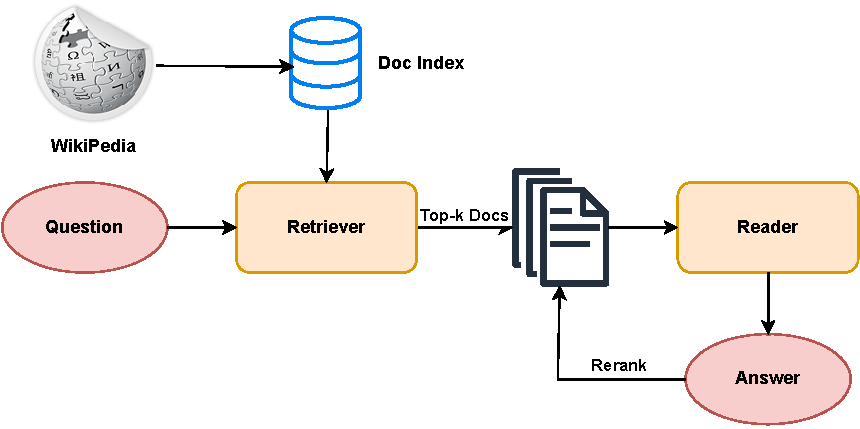
\includegraphics[
    trim={0cm 0cm 0cm 0cm},    
    clip=true
    ]{figures/my_architecture.pdf}}
    \caption{
    High-level SEAL architecture, composed of an autoregressive LM paired with an FM-Index, for which we show the first (F) and last (L) columns of the underlying matrix (more details in Sec ). The FM-index constraints the autoregressive generation (\eg, after \textit{carbon} the model is contrained to generate either \textit{tax}, \textit{dioxide} or \textit{atom} in the example) and provides the documents matching (\ie, containing) the generated ngram (at each decoding step).
    }
    \label{fig:main}
\end{figure*}

% \section{Introduction}

%here is my work
Open-Domain Question Answering (QA) is a task that aims to answer the factoid questions with amounts of documents. Previous QA systems \cite{chen2017reading} often consist of multiple components, including retriever and reader. The retriever first retrieves a small subset of the documents using the question as a query, and the reader utilize the retrieved documents as input to extract or generate the answer. 

For the purpose of enhancing the ability of the QA system, we can improve the performance of the retriever by reranking the retrieval results. Previous work \cite{karpukhin2020dense} shows that better performance in QA system can be achieved when the retrieval results are improved. Rerank the retrieval results by reranker which is a very useful approach and is wildly used after retrieval stage.

However, one limitation of the Retriever-Reranker-Reader architecture (R3) is the reranker. Conventional reranker always rerank the retrieved documents directly, it is suboptimal. Previous work  based on BERT \cite{nogueira2019passage, gao2021rethink}, rerank the retrieval documents through the questions and documents relevance. RIDER \cite{mao2021rider}  use the reader answer to rerank the documents, while it is instable.Current mainly based on seq2seq model \cite{sachan2022improving}, but is often spend much resource and time to train and inference. Therefore, we combine the answer generated by reader and the rerank model that need less resource.


%提出自己的模型
In this paper, we propose a novel Reader Help Rerank model, \system{}, which promote the QA system performance. We concatenate the question, document and answer, inputing to the \system{}, and then train the model for calculating the relevance of the question with document. At inference time, \system{} ranks the retrieved documents with the score.

We excute experiments on the Natural Questions (NQ) \cite{kwiatkowski2019natural} and TriviaQA (Trivia) \cite{joshi2017triviaqa} datasets. \system{} outperforms the state-of-the-art OpenQA systems \citep{karpukhin2020dense,sachan2021end}, and achieves EM=50 on NQ dataset and EM=51.2 on Trivia dataset. This shows the effectiveness and generalization of our approach.

Our contributions are as follows:

1. we propose \system{} to rerank the retrieved passages and achieve 10 gains in top-1 retrieval accuracy and 3 gains in QA.

2. The \system{} not only performs well on in-domain datasets, but also works well on out-of-domain datasets, showing strong generalization ability.


\section{Related Work}
Open-domain Question Answering (QA for short) requires a system to answer questions based on evidence which are retrieved from a large corpus such as Wikipedia. Current approaches consist of retriever, reranker and reader networks, where the retriever retrieves a small number of documents, and the reranker reranks the retrieved documents for the reader to answer the questions. 

\paragraph{Retriever} Text retrieval aims to find related documents from a large corpus based on a query. Earlier work \cite{chen2017reading} relied on bag-of-words-based sparse retrievers such as TF-IDF \cite{chen2017reading} and BM25 \cite{Robertson2009ThePR}. Recently,
some work improve the traditional sparse retriever with neural networks, \citet{Dai_2019} use BERT \cite{devlin2019bert} to dynamically generate term weights, and \citet                                                {mao2021generationaugmented} utilize text generation method to expand queries or documents to make better use of sparse retriever.

More recent work showed that neural retrievers can generate effective dense representations for retrieval when trained on open-domain QA datasets \cite{karpukhin2020dense}. \citet{qu2021rocketqa} improve the approach further with the hard negative sampling by iterative training. \citet{izacard2022distilling} distill knowledge from reader to retriever. There also exists some researchers focus on the pre-training of dense retrieval \cite{gao2021condenser}.

\paragraph{Reranker} Previous work showed that the pretrained language models demonstrated an outstanding capability in enhancing the performance of both sparse and dense retrievers. \citet{nogueira2019passage} present a supervised reranker for retrieval tasks based on BERT to rerank the retrieved documents. \citet{mao2021rider} propose to rerank by the reader predictions without training a new model. \citet{sachan2022improving} use a large language model as the reranker directly,  compared to the previous method. Nonetheless, it requires large amounts of computation and time at training and inference stage and performs not well as fine-tuned reranker. \citet{chuang2023expand} propose a query reranker to select the best query expand for improving document retrieval.

\paragraph{Reader} Reader models for open-domain QA are required to read multiple documents which are more than 100 documents to avoid missing the target document from the large-scale knowledge base. The reader models was divided into two primary categories, the extractive readers \cite{karpukhin2020dense}, which encode each document separately and marginalize the predicted answer probabilities and extract the answer spans from the probabilities.

While the generative readers generating the answer in a sequence-to-sequence manner,including the Fusion-in-Decoder (FiD) model \cite{izacard2020leveraging} and the Retrieval-Augmented Generation model \cite{lewis2020retrieval}. The FiD model concatenate the encoded representations of documents, which can then be decoded by the decoder and generate the answer for the query. 


\section{Method}
OpenQA aims to answer factoid questions without pre-specified domains. We assume that a large collection of documents $C$ (i.e., Wikipedia) are given as the resource to answer the questions and a retriever-reader architecture is used to tackle the task, where the retriever retrieves a small subset of the documents $D \subset C$ and the reader reads the documents D to extract (or generate) an answer. Our goal is to improve the effectiveness and efficiency of the retriever and consequently improve the performance of the reader.

In this section, we propose an optimized training approach to dense passage retrieval for open-domain QA, namely RocketQA. We first introduce the background of the dual-encoder architecture, and then describe the three novel training strategies in RocketQA. Lastly, we present the whole training procedure of RocketQA.
\subsection*{2.1 Retriever}

\subsection*{2.2 Reader}

\subsection*{2.3 Reranker}

Given an initially retrieved passage list $R$ and topN predictions of the reader $A^{[:N]}$,RIDER forms a reranked passage list $R'$ as follows. RIDER scans R from the beginning of the list and appends to $R'$ every passage  $p \in R$ if $p$ contains any reader prediction $a\in A^{[:N]}$ after string normalization (removing articles and punctuation) and tokenization.

Then, the remaining passages are appended to $R'$ according to their original order. Intuitively, if the reader prediction is perfect, the retrieval accuracy after reranking is guaranteed to be optimal. Specifically, if the reader prediction is correct, it is guaranteed that the retrieval accuracy after reranking is better, since RIDER moves all passages containing the correct answer to the top (or at least the same if those passages are all at the top before reranking). If the reader prediction is wrong, RIDER could still be better if the predicted answer co-occurs with the correct answer, the same, or worse if the predicted answer is misleading. In practice, if the reader performs reasonably well, RIDER is also likely to rerank passages well. Overall, we observe quantitatively that RIDER leads to consistent gains in terms of both retrieval accuracy and QA performance without refining the retriever (reader) or even any training itself despite the noise in reader predictions.


\bibliography{mybib}
\bibliographystyle{acl_natbib}

\FloatBarrier

\end{document}
